\documentclass{article}

\usepackage[utf8]{inputenc}
\usepackage{amsmath} % bmatrix
\usepackage{graphicx} %includegraphics

\setlength{\parindent}{1cm} % Default is 15pt.

\title{Two Dimensional Lagrangian Parcel Model with Support for Variability}

\author{Adam Abernathy\footnote{Dept. of Atmospheric Sciences, U0751826, adam.abernathy@utah.edu} \\ Jeff Fitzgerald\footnote{Dept. of Atmospheric Sciences, U0629004, j.fitzgerald@utah.edu}}

\date{\today}

\begin{document}

\maketitle

% -----------------
% Abstract
% -----------------
\begin{abstract}
Air parcel movement through the atmosphere is a key element of predicting the weather. The purpose of this project is to show an air parcel's movement through layers of the atmosphere depending on the saturation rate of the atmosphere as well as the moisture content and temperature of the parcel. 
\end{abstract}


% -----------------
% Introduction
% -----------------
\section{Introduction}

The greatest uncertainty in predicting the weather is the understanding of atmospheric moisture and its effects on an air parcel. This model will not solve the complex microphysics of cloud and parcel development but will be a simple model that shows an air parcel's vertical movement through the atmosphere. 

The American Meteorological Society (AMS) defines an air parcel as ``an imaginary volume of air to which may be assigned any or all of the basic dynamic and thermodynamic properties of atmospheric air.'' By definition a parcel is large enough to carry a significant number of molecules but still small enough where the thermodynamic properties remain uniform \cite{ams-gloss-parcel}.

This parcel model takes in a variety of parameters such as temperature, relative humidity, moisture content, and is able to model vertical motion through the atmosphere depending on the temperature and saturation level of the atmospheric layers as well as the parcel itself.

Technical descriptions of our initialization parameters are in section \ref{init-params}, return variables in section \ref{ret-vars}. You can reference a listing and technical description of internal functions used throughout the program in section \ref{comp-functions}. The core of this model is the `saturation adjustment' function which is described in moderate detail in section \ref{satadjust}.


% -----------------
% The Parcel Model
% -----------------
\newpage
\section{The parcel model program}

% -------

\subsection{Quick Start}

If you are using a UNIX/Linux environment, the ideal method of running this program is to use the included runtime script. This contains all of the initialization parameters needed to execute the program.

%It is highly recommended you maintain the most recent working version which can be downloaded from https://github.com/whokilledkermit/parcel\_model .

\begin{verbatim}
run_p_model.csh
\end{verbatim}

% -------

\subsection{Initialization parameters}

The following parameters are needed to run the parcel model. These parameters set how many trials we run, if the user wants to save the output and print it to the console, and change the perturbation scalar among other options.

\begin{enumerate}

\item \{do\_write\_output\}, defines if the user wants to save the output where a value of `1' will store the data and `2' will not.

\item \{do\_console\_output\}, asks if the user wants to print the results to the console. The parameters options are the same as \{do\_write\_output\}.

\item \{pert\_scalar\}, defines the perturbation scale. In other words, this defines how much variability we want the parcel to have where a value of `1' is the largest amount of variability for the parcel and `0' is no variability.

\item \{n\_trials\}, the initialization parameter for the number of trials we want to run for the parcel.

\end{enumerate}

\subsection{Defining Initial parcel properties}\label{init-params}
At initialization we must define all of our initial parcel properties. Below are the default parameters included \cite{krueger}. 

\begin{enumerate}
\item \{pMB\} = 1000 [mb], initial sea level pressure
\item \{TC\} = 20.0, initial sea level temperature in degrees Celsius
\item \{qv\} = 14.8e-3, initial water vapor mixing ratio
\item \{qc\} = 0.0, adjusted mixing liquid water ratio which hasn't been calculated yet
\item \{qw\} = 14.8e-3, initial liquid water mixing ratio
\item \{qvs\} = 0.0, initial saturation mixing ratio
\item \{rh\_i\} = 0.5, initial relative humidity (deactivated in ver R4-Build-2)
\item \{dpMB\} = 10.0, pressure intervals
\item \{ptopMB\} = 500.0, final pressure height
\end{enumerate}

% -----------------
% Governing Equations
% -----------------

\newpage
\section{Governing principals and model results}

\subsection{Return Variables}\label{ret-vars}
These are the results that are returned after the program is executed.

\begin{enumerate}

\item \{theta\}, Adjusted potential temperature in degrees [K]
This is the temperature a parcel would have if it became dry(or unsaturated) and was brought down the dry adiabat to sea level pressure (or $\approx$ 1000 mb).

\item \{qv\}, Adjusted mixing water vapor Ratio in [Kg/Kg]. This is the ratio of Water Vapor (gas) to air.

\item \{qc\}, Adjusted mixing liquid water ratio in [Kg/Kg].This is the ratio of Liquid Water to air.

\item \{qvs\}, Saturation mixing ratio in [Kg/Kg]. The amount of water vapor in the air if an air parcel was fully saturated and could not hold any more water.

\item \{pibar\}, Exner Function $\left(\bar{\Pi}\right)$. This is a non-dimensional pressure that help us compute the temperature moving forward. The bar indicates that this is a value with respect to the environment rather than the parcel.

\end{enumerate}


% -----------------
% Computational Functions
% -----------------
\newpage
\section{Computational Functions}\label{comp-functions}

Technical description of the computational functions and their purpose. 

% -------

\subsection{Potential temperature ($\Theta$)}
\begin{verbatim}
compute_theta.cpp
\end{verbatim}

This equation is where we compute the initial potential temperature ($\Theta$) with the input variables of temperature (T) and pressure (p) \cite{wallace}.

\begin{equation}
\Pi = \left(\frac{p}{p_{0}}\right)^{\frac{R}{C_{p}}}
\end{equation}

Where $\Pi$ is the Exner function, we yield \cite{krueger}

\begin{equation}
\Theta = \frac{T}{\Pi}
\end{equation}

% -------

\subsection{Compute water vapor saturation}
\begin{verbatim}
compute_esat_pa.cpp
\end{verbatim}

This calculates the saturation water vapor pressure over water in Pascals with the input variable of temperature (T). We are using a Taylor expansion. The Taylor expansion is broken up into parts where (-) and (+) symbols are used to denote the sign of the computations.

\begin{eqnarray}
e_{s} &=& 23.832241 \\
&-& 5.02808 \times \log_{10}\left(T\right) \nonumber \\
&-&\left(1.3816 \times 10^{-7}\right)\left(10exp\left(11.344 - 0.0303998T\right)\right) \nonumber \\
&+&\left(8.1328 \times 10^{-3}\right)\left(10exp\left(3.49149 - \frac{1302.8844}{T}\right) - 10exp\left(\frac{2949.076}{T}\right)\right) \nonumber
\end{eqnarray}

% -------

\subsection{Change in saturation water vapor}
\begin{verbatim}
compute_des_dt_pa.cpp
\end{verbatim}

This calculates the change in saturation water vapor pressure over water in pascals. Input variable includes temperature (T).

\begin{equation}
\frac{d_{es}}{dt} = \frac{L}{R_{v}}\left(\frac{e_{s}\left(T\right)}{T^{2}}\right)
\end{equation}

where $L$ and $R_{v}$ are thermodynamic constants\footnote{See equation 13 from \cite{krueger}}.

\subsection{Alpha}
\begin{verbatim}
compute_alpha.cpp
\end{verbatim}

In order to solve the following system of equations

\begin{equation}
\alpha \equiv {
\begin{cases}
&\Theta\\% = \text{Potential temperature}\\
&w\\% = \text{Mixing Ratio}\\
&w_{1} \equiv \text{Taylor expansion of $w_{s}$(T)}
\end{cases}
}
\end{equation}

we can algebraically  solve them using the function $\alpha$ \cite{krueger}.

\begin{equation}
\alpha\left(T,p\right) = \frac{\frac{de_{s}}{dt}\left(0.622\right)\bar{\Pi}\bar{p}}{\left[\bar{p}-e_{s}\left(T^{*}\right)\right]^{2}}
\end{equation}

% -------

\subsection{Result data storage}
\begin{verbatim}
write_output.cpp
\end{verbatim}

This function takes the computational output and writes it to a comma separated values (CSV) file which is useful for diagnostics and necessary to plot the parcel's motion through the atmosphere. 

By default the model stores the results as \texttt{results.txt}. You can modify this filename by editing the filename passed to this function in the \texttt{main()} routine. Future versions of this program should include the support for user defined output files.

% -------

\subsection{Parcel Motion Driver}
\begin{verbatim}
parcel_motion_driver.cpp
\end{verbatim}

This function is what simulates the parcel to move up and down in the atmosphere. It creates a loop that runs through a number of iterations which will drive the parcel in a given vertical direction. It stores these results in an array which are then used to drive the parcel up and down through the atmosphere depending on the values in the array. The driver takes in initialization parameters and calls the saturation adjustment which returns the parcel's new state for the given pressure level. The driver will iterate until it reaches the top or bottom of the atmosphere. It then prints out the results to the user.

% -------

\subsection{Terminal Library}
\begin{verbatim}
terminal_lib.cpp
\end{verbatim}

This function prints the parcel values to the screen of the terminal. It prints when the parcel is descending as well as each of the parcel's values as it descends through the atmosphere. 


% ------------
% Saturation Adjustment
% ------------

\section{Saturation Adjustment}\label{satadjust}
\begin{verbatim}
satadjust.cpp
\end{verbatim}

The primary algorithm that performs an isobaric moist adiabatic adjustment. The final state is either sub-saturated with no liquid water present or exactly saturated with liquid water present.

\subsection{Input Parameters} 
This function takes in three parameters which are:

\begin{enumerate}
\item \{theta\}, potential temperature
\item \{qv\}, mixing ratio of water vapor
\item \{qc\}, mixing ratio of liquid water
\end{enumerate}


\subsection{Output Parameters}
The output parameters are:

\begin{enumerate}
\item \{theta\}, adjusted potential temperature
\item \{qv\}, adjusted mixing ratio of water vapor
\item \{qc\}, adjusted mixing ratio of liquid water (kg/kg)
\item \{qvs\}, saturation mixing ration
\item \{pibar\}, Exner function with respect to the environment
\end{enumerate}

\subsection{Methodology}
The actual workings of the saturation adjustment are rather complicated. Fig \ref{fig:satadjust} shows a simple schematic of the process.

\begin{figure}
\centering
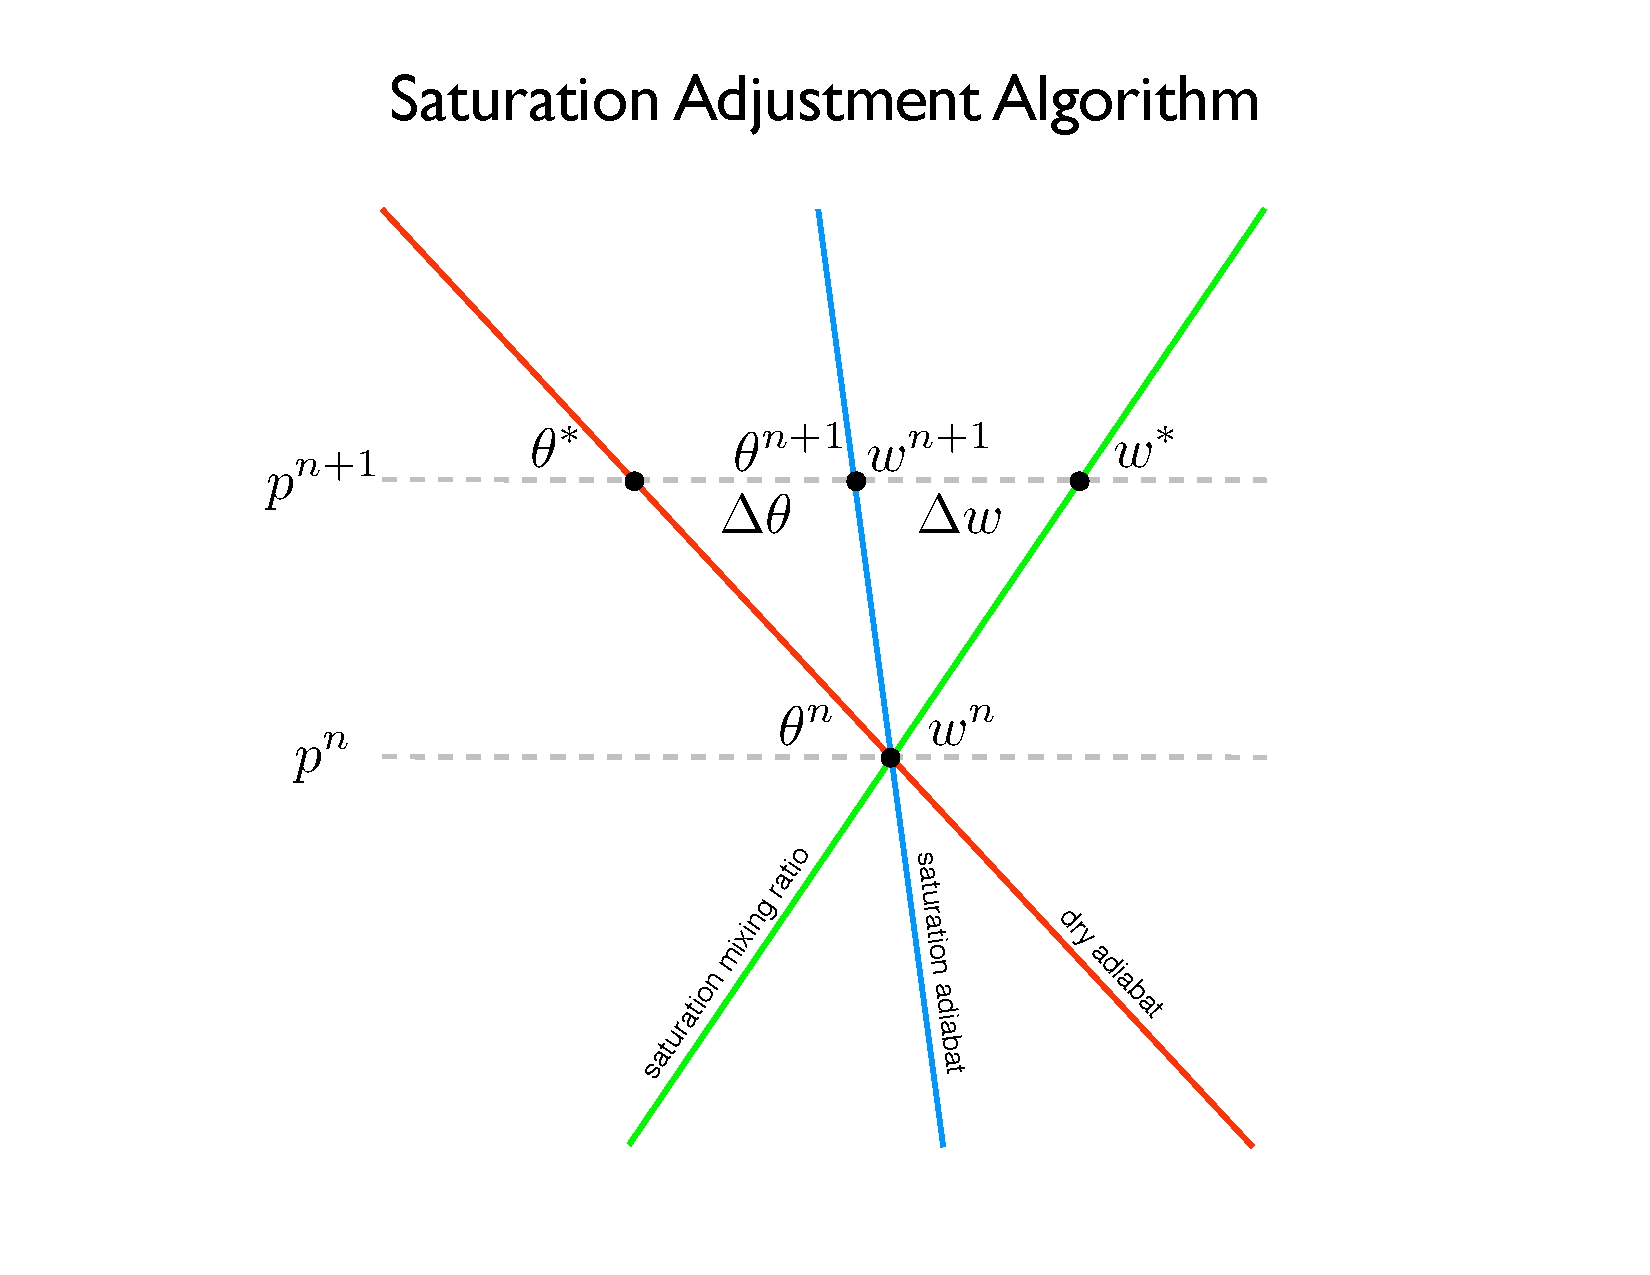
\includegraphics[width=4.5in]{satadjust.pdf}
\caption{This schematic shows geometrically the processes of the saturation adjustment \cite{krueger}.}
\label{fig:satadjust}
\end{figure}


% -----------------
% Program Design
% -----------------
\newpage
\section{Program Design}

The general workflow of the parcel model is described by Fig \ref{fig:programflow}.

\begin{center}
\begin{figure}[h]
\centering
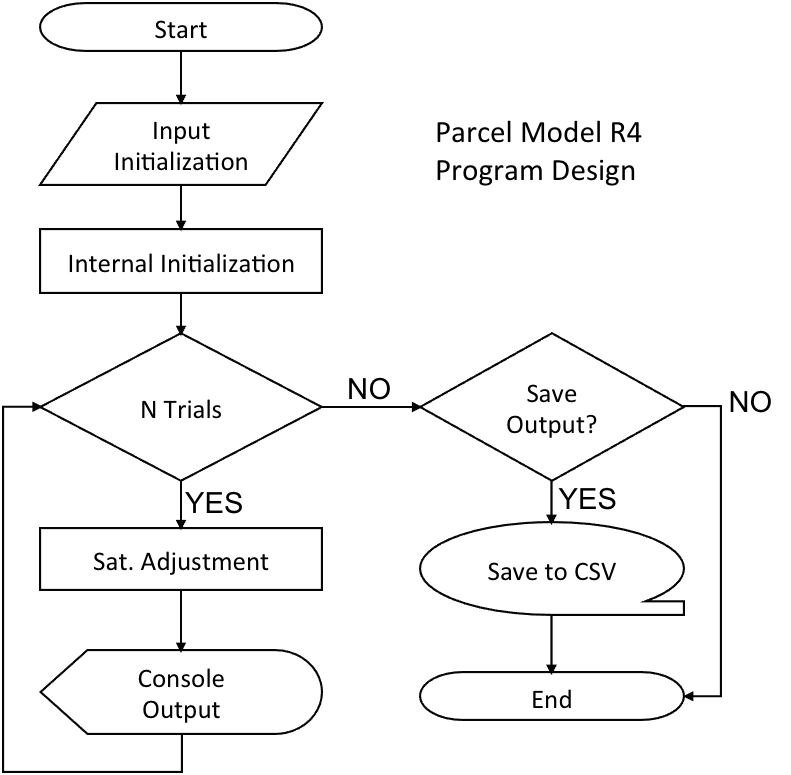
\includegraphics[width=3.5in]{program_flow}
\caption{General schematic of program workflow.}
\label{fig:programflow}
\end{figure}
\end{center}






% -----------------
% How we divided the work
% -----------------
\newpage
\section{How the  work was divided}

Of the computational functions, Adam Abernathy wrote the parcel motion driver, output writer, terminal library, saturation adjustment and the Newton Method. Jeff Fitzgerald wrote the potential temperature, compute water vapor saturation, change in saturation water vapor, alpha method. The read.me file was created by Adam Abernathy while the documentation was created by Jeff Fitzgerald. Both Adam and Jeff edited each others parts of the project.


% -----------------
% Future Work
% -----------------
\newpage
\section{Future work}
Our ultimate goal was to incorporate variability of all our parameters such as relative humidity, temperature, saturation vapor pressure, etc. We were unable to incorporate all of this variability and for this project we were only able to add variability to temperature. Future work should extend the variability to all aspects of the atmosphere to show a more accurate representation of an air parcel's motion through the atmosphere.

\section{Acknowledgements}
We would like to think Professor Steve Krueger, Dept. of Atmospheric Sciences, for all of his contributions on developing the saturation adjustment algorithm and his insight into understanding thermodynamic properties of the atmosphere.

\newpage
\begin{thebibliography}{4}

\bibitem{ams-gloss-parcel}
Am. Met. Soc.
\emph{American Meteorological Society Glossary of Meteorology},\\
http://glossary.ametsoc.org/wiki/Air\_parcel

\bibitem{krueger}
Steve Krueger.
\emph{Introduction to Cloud Physics},
ATMOS 5200. University of Utah, Salt Lake City. Fall 2014 \\
http://www.inscc.utah.edu/~krueger/5200

\bibitem{rogers}
R. R. Rogers and M. K. Yau.
\emph{A Short Couse in Cloud Physics},
Elsevier Books (1989)

\bibitem{wallace}
John Wallace and Peter Hobbs.
\emph{Atmospheric Science An Introductory Survey},
Elsevier Books (2006)



\end{thebibliography}


\end{document}